
\begin{frame}
    \frametitle{Protective Master Boot Record}
    \framesubtitle{Motivation}

    \begin{itemize}
        \item Master Boot Record (MBR): Älterer Standard für Partitionstabellen.
        \item Ältere Systeme / Programme unterstützen nur MBR.
    \end{itemize}

    \vspace{0.5cm}

    \begin{alertblock}{Gefahr von Datenverlust}
        \begin{itemize}
            \item MBR in LBA 0 erwartet.
            \item Ansonsten: Nicht / fehlerhaft partitioniert.
            \item Datenträger wird ggf. neu formatiert.
            \item Partitionsinformationen werden überschrieben.
        \end{itemize}
    \end{alertblock}
\end{frame}

\begin{frame}
    \frametitle{Protective Master Boot Record}
    \framesubtitle{Funktionsweise}

    \begin{itemize}
        \item MBR-Partitionstabelle mit einer Partition.
        \begin{itemize}
            \item Alte Systeme: Partitionsinformationen sind gültig.
        \end{itemize}
        \item Partition belegt den ganzen Datenträger.
        \begin{itemize}
            \item Alte Systeme: Kein freier Speicher vorhanden.
        \end{itemize}
        \item Tatsächliche Partitionsinformationen werden "geschützt".
    \end{itemize}
\end{frame}

\begin{frame}
    \frametitle{Protective Master Boot Record}
    \framesubtitle{Beispiel}

    \centering
    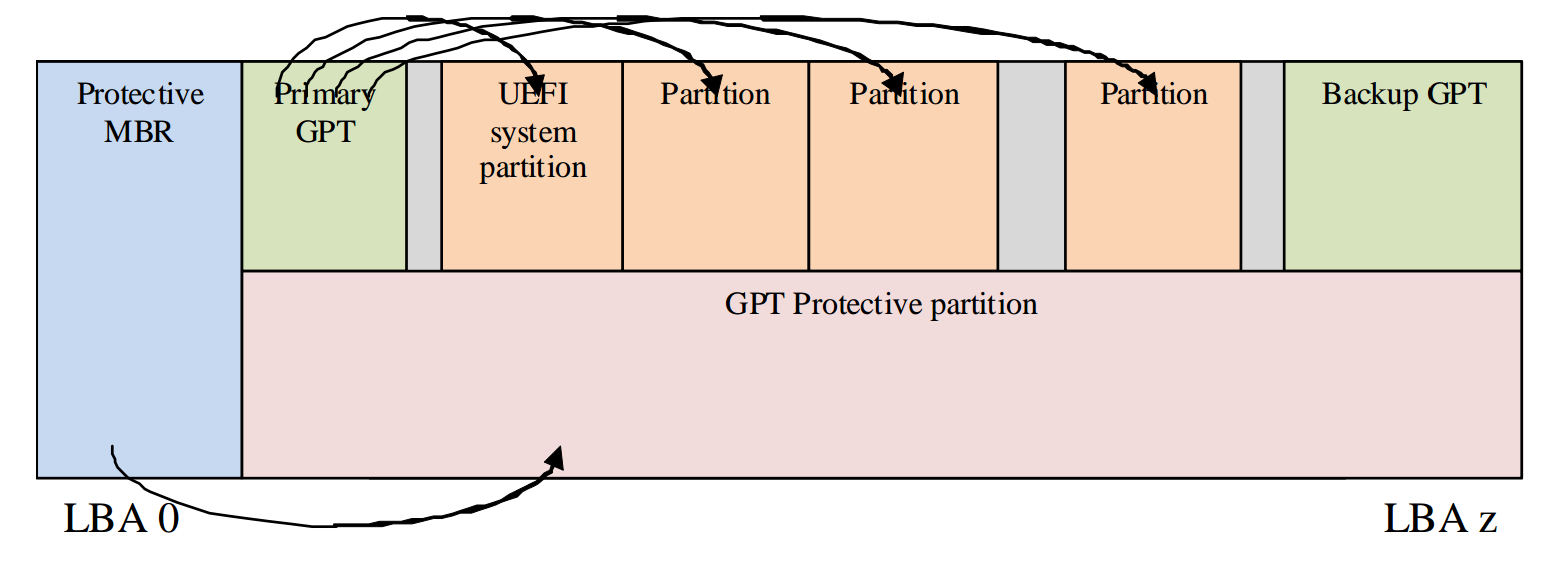
\includegraphics[width=\textwidth]{content/graphics/GPT_Layout_with_protective_MBR.png}
\end{frame}
